\cleartooddpage[\thispagestyle{empty}]
\chapter{Sample Code}\label{APPENDIXB}

The method for vortex identification for this study is a modification from previous work\cite{sunderland2016vortex}. The calculation of vortex cores was based on in-house C++/Python codes derived from the open-source Vascular Modelling ToolKit (VMTK) \cite{antiga2004robust}. Prior to any calculations, velocity data is first re-sampled onto a rectilinear grid whose voxel size is 0.2mm. \newline
\underline{In the first step,} the classic $\lambda_2$ method by Jeong and Hussain \cite{jeong1995identification} was used to define the negative $\lambda_2$ region (\textit{i.e} $\lambda_2 < 0$). Then, \underline{in the second step}, vortex core lines were estimated by the method proposed by Sujudi and Haimes \cite{sujudi1995identification}. In essence, in the negative $\lambda_2$ region, a local velocity vector $\overline{v}$ lies along a vortex core line if the following two conditions hold: (1) the 3 $\times$ 3 spatial gradient matrix of $\overline{v}$ has two complex eigenvalues and one real eigenvalue and (2) the 3 $\times$ 3 spatial gradient matrix of $\overline{v}$ has an eigenvector $\vec{\alpha}$ corresponding to the above-mentioned real eigenvalue. Now, if we define a new scalar value \textit{K} as follows,

	\begin{equation}
	K(x,y,z) =
	\begin{cases}
	|dot(\overline{v},\vec{\alpha})|, & if \text{ $\lambda_2$}  < 0 \\
	0, & Otherwise
	\end{cases}
	\end{equation}
where $|\cdot|$ is an absolute operator. Of note, in Eqn. 2, both the $\overline{v}$ and $\vec{\alpha}$ are normalized and therefore, the scalar field \textit{K} defined above is bounded between 0 and 1. If the \textit{K(x,y,z)} is close to 1 then the location \textit{(x,y,z)} is within the proximity of the vortex core line as suggested by Sujudi and Haimes \cite{sujudi1995identification}. 

\begin{figure}[t]
\begin{center}
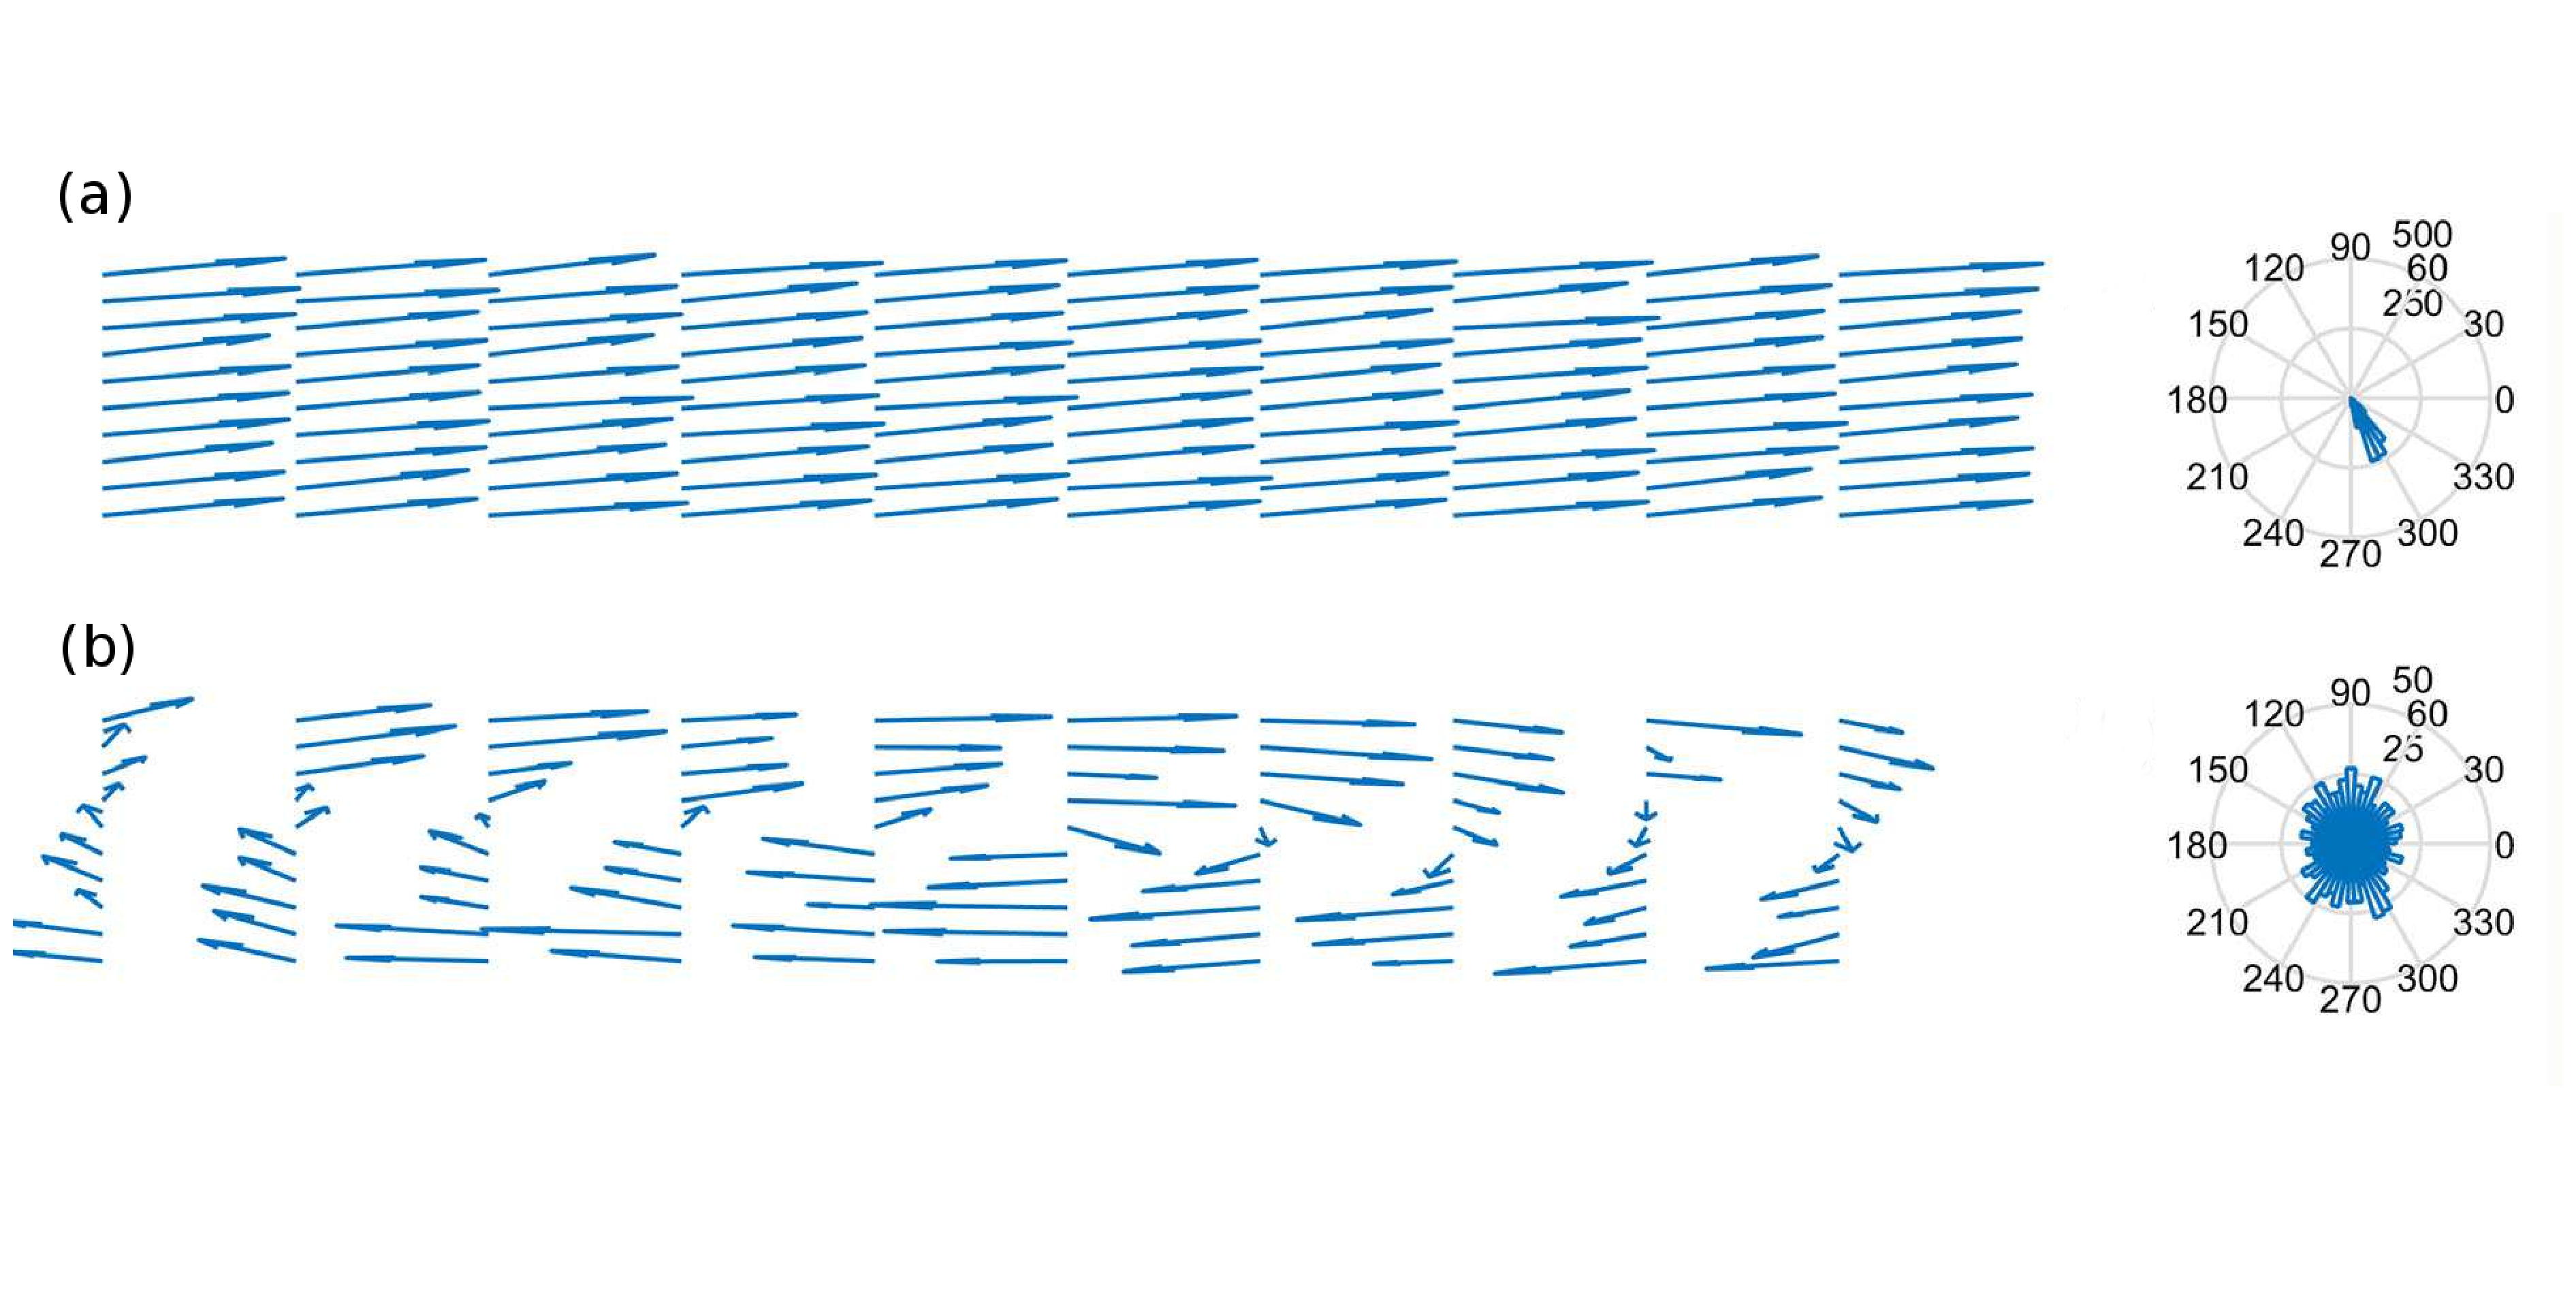
\includegraphics[width=3.0in]{BIO-17-1393_fig_9.eps}
\end{center}
\caption{Two examples illustrating the relationship between the angular histogram and NE: (a) a simple laminar flow case and (b) a rotational flow (eddy) case. In both cases, the right and left plots are the vector flow field and the histogram of angular vector direction, respectively. Vector fields were decimated by a factor of 3 for better visualization.}
\label{NE} 
\end{figure} 
	
\underline{In the third step}, we calculated local normalized entropy (NE) of velocity directions \cite{shannon2001mathematical} following work in the flow visualization literature (e.g. \cite{xu2010information,ma2014graph}). The \textit{NE} is close to 0 if the velocity direction closely concentrates one value out of \textit{N} possible values (see Fig. ~\ref{NE}(a); NE=0.05). In contrast, the entropy measure \textit{NE} becomes 0.95 if the probability of velocity directions is almost equally likely, as shown in Fig ~\ref{NE}(b). Given an arbitrary vexel located at \textit{(x,y,z)} within the dome of an IA, we selected a fixed volume of interest (VOI; $N_x$ x $N_y$ x $N_z$; $N_x=N_y=N_z=11$ in this study) centered at the voxel. One additional metric \textit{H(x,y,z)} can be obtained by combining \textit{K(x,y,z)} together with the \textit{NE(x,y,z)} as follows,
	\begin{equation}
	H(x,y,z) = K(x,y,z) * NE(x,y,z)
	\end{equation}
\textit{H(x,y,z)} is a scalar field representing the likelihood of residing within a vortex core region for a location (\textit{x,y,z}). \textit{H} also has a normalized range between 0 and 1. Thus, based on a fixed threshold, the vortex core region in this study can be obtained using the classic Marching-cube method \cite{lorensen1987marching}. in this study, 0.30 was used as the threshold for all data sets.

\section{HelloWorld.c}\label{APPENDIXB_SECTION1}
\renewcommand{\baselinestretch}{1.25}
\lstset{
  language=c
}
\lstinputlisting{Appendices/HelloWorld.c}
\renewcommand{\baselinestretch}{\lineheight}
